% C original page filename: codex/H134-06/pages/H134-06_134-2_scan182.tex
\scanpage{182}\mspage{37}%
% archive sheet number: 182
% L1a: raised parenthesis, with a long attachment guide entering after profinis.
the ``profinite completions'' \inserted{(in the sense of Artin-Mazur)} prime to $p$ (the characteristic of $k$) of such spaces.
One sees clearly how to \unsure{approach} such a programme in characteristic $0$, but one foresees additional amusement, or even mystery, in characteristic $p>0$, for varieties which, even birationally, would refuse to let themselves be lifted to characteristic $0$!

% Separate rule: whole-image endpoints approximately (688,720) and (976,715).
\figure{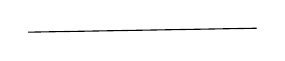
\begin{tikzpicture}
\draw[line width=0.4pt] (0,0) -- (2.9,0.05);
\end{tikzpicture}}

From these essentially geometric cogitations, I could not at present draw a precise programme for the development of algebraic structures adequate to express them.
I shall confine myself to a few remarks in the margin.

\deleted{\unsure{a|$\alpha$})} For a long time I have been \unsure{intrigu-|intrigued} by the idea of a ``linearization'' of an (ordinary) homotopy type, i.e. the question of the type: If $X$ is a homotopy type, how much cohomological information of the type: cohomology of $X$ with variable coefficients $M$ (constant%
% Compact detached point near (818,1807), below the first constant; physical presence retained, origin unassigned.
\raisebox{0pt}[0pt][0pt]{\parbox{0pt}{\figure{\begin{tikzpicture}[overlay,x=1pt,y=1pt]
\fill (-28,-7) circle[radius=0.35pt];
\end{tikzpicture}}}} or twisted constant),
% A detached short vertical mark at approximately (271,1837), above the beginning of structure; origin uncertain.
\raisebox{2.2ex}[0pt][0pt]{\parbox{0pt}{\figure{\begin{tikzpicture}[overlay]
\draw[line width=0.3pt,line cap=round] (0.16,0) -- (0.17,-0.04) -- (0.17,-0.06) -- (0.18,-0.06);
\end{tikzpicture}}}}multiplicative structure
% The two short overwritten strokes favour = over +; the underlying sign remains doubtful.
% A distinct compact point at approximately (1024,1876), below the first H crossbar, is drawn without assigning it a mathematical role.
$\deleted{\unsure{=|+}}\raisebox{0pt}[0pt][0pt]{\parbox{0pt}{\figure{\begin{tikzpicture}[overlay]
\fill (0.09,0.05) ellipse [x radius=0.012cm,y radius=0.02cm];
\end{tikzpicture}}}}H^i(X,M)\times H^j(X,N)\mathrel{\unsure{\dashv|\to|-}}H^{\unsure{i\cdot j|i+j|ij}}(X,M\otimes N)$,
plus possibly other cohomological operations -- is it%
% Detached short hooked stroke at approximately (1619,2077), well to the right of est-il; no word or punctuation function assigned.
\raisebox{0.4ex}[0pt][0pt]{\parbox{0pt}{\figure{\begin{tikzpicture}[overlay]
\draw[line width=0.3pt,line cap=round] (0.25,0) -- (0.27,-0.07) -- (0.31,-0.12);
\draw[line width=0.3pt,line cap=round] (0.27,-0.05) -- (0.26,-0.09);
\end{tikzpicture}}}} necessary to have in order to \unsure{reconstruct|reconstruct} the homotopy type entirely \deleted{\unsure{?}}? (say,
